\documentclass[../main.tex]{subfiles}

\begin{document}
    
\chapter{Candidate Universe Ranking}
    
Following the successful derivation of an objective sector classification heuristic (addressing RG-1), the next step is to derive a methodology to rank our sectors against each other, to isolate the optimal sector/sectors, without imposing any subjective criteria on the selection. Thus, this section begins the discussion of addressing the second research goal, RG-2 (see Section~\ref{research_goals:specific_research_goals}):

\begin{table}[h!]
    \centering
    \begin{tabular}{| c | c |}
        \hline
        &  \\
        RG-2 & Rank candidate sector universes against each other using entirely objective criteria. \\
        & \\
        \hline
    \end{tabular}
    \caption{Specific project research goal RG-2.}
    \label{table:candidate_universe_ranking:research_goal}
\end{table}

\section{Sample Learned Sector Universe}

\begin{wrapfigure}[18]{r}{0.5\textwidth}
    \centering
    \vspace{\wrapfigadjustment}
    \fbox{
    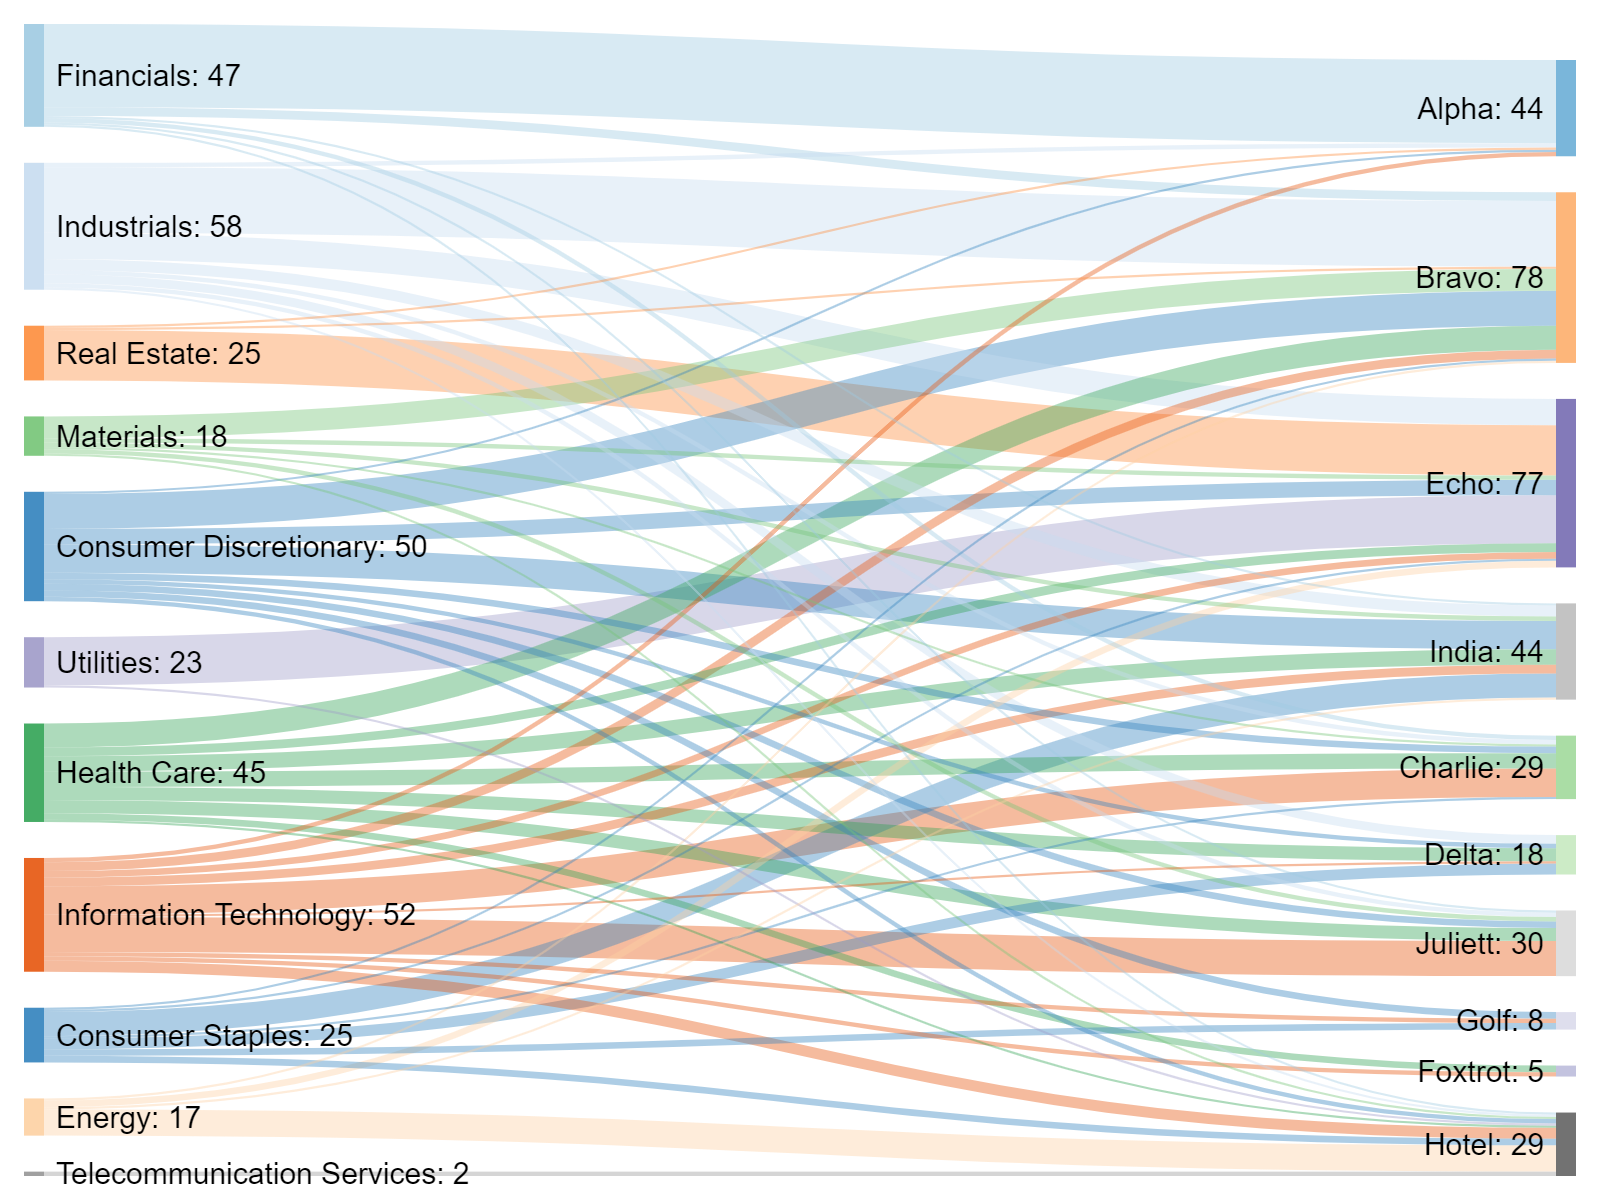
\includegraphics[width=0.48\textwidth]{images/sample_ls_universe.png}
    }
    \caption{Sample learned sector universe - Ward Linkage; 2010 Data; 10 Sectors.}
    \label{fig:candidate_universe_ranking:sample_ls_universe}
\end{wrapfigure}

To best motivate the approach we decided to use when comparing and ranking candidate sector universes, it is worthwhile to discuss an example.

Figure~\ref{fig:candidate_universe_ranking:sample_ls_universe} is a Sankey Diagram, representing the new learned sector assignments of various corporations from our search space by means of comparison to the benchmark. The left-hand side of the diagram represents the original benchmark sectors, and their constituent assets, while the right hand side represents the new learned sector assignment of the same assets.

As evidenced by the diagram, there appears to be significant transitory behavior of corporations across sectors when comparing the benchmark sectors to the learned sectors. Additionally, there also appears to be a significant amount of mixing between the sectors, with very few sectors appearing to be preserved between the sector universes. In the example, the only sector that can be considered remotely similar to a benchmark sector would be learned sector \textit{Alpha} to benchmark sector \textit{Financials}.

Other sectors however, appear largely broken up and dispersed when comparing their benchmark sector to the new learned sector univese. Particularly noticable examples of this include the benchmark sectors \textit{Health Care}, \textit{Information Technology}, and \textit{Consumer Discretionary}. Due to the fundamentals-driven nature of our classification heuristic, this result is not entirely surprising; the benchmark sectors that appear to have the most dispersion in the learned sector universe are ones which are increasingly integral to regular business, regardless of sector; particularly \textit{Information Technology}.

As illustrated in this section with a single example, there is extremely little congruity between the benchmark sector classification and the learned sector classification. This pattern can be observed across a larger set of learned sector universes in Figure~\ref{fig:hierarchical_clustering_model:partial_search_space}, a partial visualization of the learned sector search space.

Due to this fact, is would be extremely difficult to perform a sector-by-sector analysis across sector universes as a means for comparison. There is obvious difficulty in matching sectors across universes (as illustrated by the example in Figure~\ref{fig:candidate_universe_ranking:sample_ls_universe}) without introducing significant bias to the comparison metric. Furthermore, there is an additional issue presented by the fact that the number of sectors in two given candidate learned sector universes may not be identical (let alone the number of constituent corporations in a given sector), thus completely prohibiting a sector-by-sector analysis.

To combat this issue, we decided to evaluate the sector universes as a whole, and then analyze universe-level metrics to rank the candidate learned sectors. To this end, we developed \textit{reIndexer}, which is discussed at length in the following section.

\end{document}